\documentclass{article}
\pagenumbering{gobble}
% \usepackage[bibstyle=phys,citestyle=numeric-comp,biblabel=brackets,sorting=none,backend=biber,bibencoding=auto]{biblatex}
% \addbibresource{references.bib}
% \DeclareFieldFormat{titlecase}{#1}%turn off sentence case

% \DeclareSourcemap{
%   \maps[datatype=bibtex, overwrite]{
%     \map{
%       \step[fieldset=extra, null]
%       \step[fieldset=note, null]
%     }
%   }
% }

% \usepackage{placeins}
% \usepackage{flafter}
% \usepackage[utf8]{inputenc}
\usepackage{mlmodern}
\usepackage[T1]{fontenc}

% \usepackage[english]{babel}
\usepackage{amsmath,amsfonts,amssymb}
\usepackage{mathrsfs}
\usepackage{clock}
\usepackage[clock]{ifsym}
% \usepackage{mathtools}
\usepackage{dcolumn}% Align table columns on decimal point
\usepackage{bm}
\usepackage[dvipsnames]{xcolor}
\usepackage{graphicx} % Allows for eps images
\usepackage{array}
\newcolumntype{C}[1]{>{\centering\let\newline\\\arraybackslash\hspace{0pt}}m{#1}}
\newcolumntype{L}[1]{>{\raggedright\let\newline\\\arraybackslash\hspace{0pt}}m{#1}}
\newcolumntype{M}[1]{>{\let\newline\\\arraybackslash\hspace{0pt}}m{#1}}
\usepackage{caption}
\usepackage{subcaption}
% \usepackage[caption=false,justification=justified]{subfig}
% \usepackage{authblk}
% \usepackage[framed, numbered]{matlab-prettifier}
\usepackage{float}
\usepackage{ragged2e}
% \usepackage{nidanfloat}
% \usepackage{stfloats}
% \usepackage{fixltx2e}
% \usepackage{url}
\usepackage{enumitem}
\usepackage{tensor}
\usepackage{centernot}
\usepackage{dsfont}
\usepackage[mathlines]{lineno}
% \linenumbers\relax % Commence numbering lines
% \usepackage[subfigure]{tocloft}
\usepackage{csquotes}
\usepackage{tikz}
\usetikzlibrary{shapes}
% \usetikzlibrary{quantikz}
\usetikzlibrary{arrows}
\usetikzlibrary{arrows.meta}
\usetikzlibrary{calc}
\usetikzlibrary{decorations.markings}
\usepackage{pgfplots}
\usepackage[outline]{contour}
\usepackage{tikz-feynman}
\usepackage{etoolbox}
% \usepackage{hyperref}
% \hypersetup{colorlinks=true,hyperfootnotes=false}
\pgfplotsset{compat=newest}
%\pgfplotsset{compat=1.17}
\usepackage[framemethod=tikz]{mdframed}
\definecolor{boxcolor}{HTML}{F5F5F5}

\renewenvironment{quote}%
  {\list{}{\leftmargin=-1.0em\rightmargin=-1.0em}\item[]}%
  {\endlist}

\def\QuantikzSeparationRow{0.8}

\usepackage{xparse}
\ExplSyntaxOn
\DeclareExpandableDocumentCommand{\IfNoValueOrEmptyTF}{mmm}
 {
  \IfNoValueTF{#1}{#2}
   {
    \tl_if_empty:nTF {#1} {#2} {#3}
   }
 }
\ExplSyntaxOff

\usepackage{xstring}
\def\replace#1#2#3{%
 \def\tmp##1#2{##1#3\tmp}%
   \tmp#1\stopreplace#2\stopreplace}
\def\stopreplace#1\stopreplace{}

\newcommand{\ChangeGreek}[1]{\begingroup
\let\theta\Theta
#1
\endgroup}

% Fix for spacing around \left and \right
% see: https://tex.stackexchange.com/questions/2607/spacing-around-left-and-right
\let\originalleft\left
\let\originalright\right
\renewcommand{\left}{\mathopen{}\mathclose\bgroup\originalleft}
\renewcommand{\right}{\aftergroup\egroup\originalright}

\definecolor{primarycolour}{HTML}{2266C0}
\definecolor{secondarycolour}{HTML}{B10061}
\definecolor{tertiarycolour}{HTML}{7000CC}
\definecolor{quaternarycolour}{HTML}{008A8A}
\newcommand{\ColA}{primarycolour}
\newcommand{\ColB}{secondarycolour}
\newcommand{\ColC}{tertiarycolour}
\newcommand{\ColD}{quaternarycolour}

% \input{macros.tex}

\DeclareDocumentCommand\Controlled{ m o o o }{
    \IfNoValueOrEmptyTF{#2}{}{\Control^{#2}}
    \IfNoValueOrEmptyTF{#3}{}{\Anticontrol^{#3}}
    \IfNoValueTF{#4}{#1}{{#1}^{#4}}
}
\tikzstyle{phantomhelper} = [
    rectangle,
    draw=none,
    fill=white,
    sloped,
    inner sep=0pt,
    outer sep=0pt,
    minimum width=3.75mm,
    minimum height=2.75mm,
]

\pgfplotscreateplotcyclelist{custom-list}{
    {cyan!0!magenta,mark=*},
    {cyan!33!magenta,mark=square*},
    {cyan!66!magenta,mark=triangle*},
    {cyan!100!magenta,mark=diamond*}%
}

%%% Wormhole mouths diagram:
\def\w{1}
\def\x{2}
\def\y{0.1}
\def\z{0.2}
\def\radius{1.625}
\def\sep{3}

% Style to set camera angle, like PGFPlots `view` style
\tikzset{viewport/.style 2 args={
    x={({cos(-#1)*\radius cm},{sin(-#1)*sin(#2)*\radius cm})},
    y={({-sin(-#1)*\radius cm},{cos(-#1)*sin(#2)*\radius cm})},
    z={(0,{cos(#2)*\radius cm})}
}}

% Convert from spherical to cartesian coordinates
\newcommand{\ToXYZ}[2]{
    {sin(#1)*cos(#2)}, % X coordinate
    {cos(#1)*cos(#2)}, % Y coordinate
    {sin(#2)}          % Z (vertical) coordinate
}

\def\rotation{20}
\def\offset{37.5}

%%% Penrose diagram:
% \usepackage{xparse} % Already included above as required for other purposes
\ExplSyntaxOn
\DeclareExpandableDocumentCommand{\eval}{m}{\fp_eval:n {#1}}
\ExplSyntaxOff

\tikzset{->-/.style={decoration={markings, mark=at position #1 with {\arrow{Latex[length=2.75mm,width=1.5mm]}}},postaction={decorate}}}

\def\sizing{10}%keep=10
\def\scaling{0.025}%fixed=0.025
\def\num{32}%25~101, test=5, good=32, okay=24
\def\spacing{0.035}%keep=0.0325~4, good=0.035
\def\domain{2.25}%min=1, max=10, fair=5, good=2.25
\def\granularity{129}%min=257, best=2049, test=17, good=129
\def\tension{0.5}
\def\bound{\eval{\scaling*(atand(\sizing*\domain)+atand(\sizing*\domain))}}
% Convert from Minkowski to Penrose-Carter coordinates
\newcommand{\ToUV}[2]{
    {\scaling*(atan(\sizing*(#1+#2))+atan(\sizing*(#1-#2)))},% T coordinate
    {\scaling*(atan(\sizing*(#1+#2))-atan(\sizing*(#1-#2)))} % X coordinate
}

%%% Bloch sphere:
\usepackage{blochsphere}
\usetikzlibrary{positioning,arrows,calc,math,angles,quotes}
\def\rotationSphere{-90}
\def\radiusSphere{2cm}
\def\psiLat{45}
\def\psiLon{45}

\input{./../../preamble/macros.tex}

\renewcommand{\large}{\normalsize}

% \usepackage{geometry}
% \geometry{
% paperwidth=8cm,
% paperheight=8cm,
% margin=0cm
% }

\begin{document}
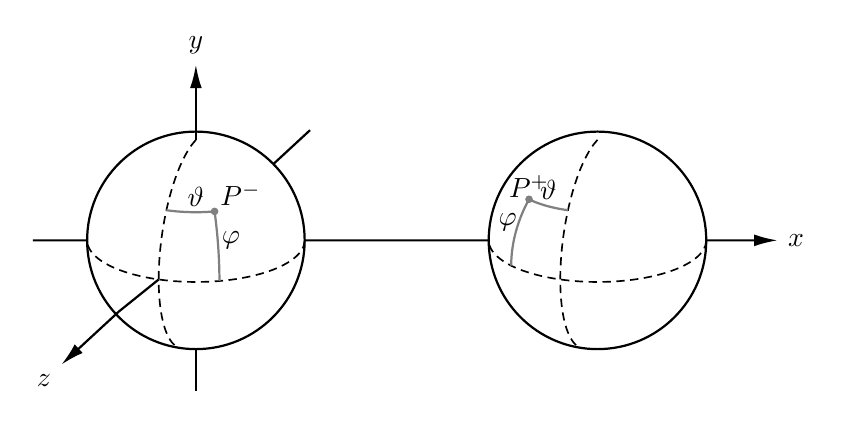
\begin{tikzpicture}[scale=0.85]
    \iffalse
    % Draw shaded circle that looks like a sphere
    \begin{scope}
       \clip (0,0) circle (1);
    \begin{scope}[transform canvas={rotate=-\rotation}]
    \shade [ball color=white] (0,0.5) ellipse (1.8 and 1.5);
    \end{scope}
    \end{scope}
    \fi
    
    \begin{scope}[viewport={\rotation}{22.5},shift={(-\sep cm,0)}]
    
    \draw[thick] (\ToXYZ{270-\rotation}{0}) -- ++($0.5*(\ToXYZ{270-\rotation}{0})$);
    \draw[-{Latex[black,length=3mm,width=1.5mm]},thick] (\ToXYZ{90-\rotation}{0}) -- ++($\sep*(\ToXYZ{90-\rotation}{0})$) -- ++($1.35*(\ToXYZ{90-\rotation}{0})$) node[right, font=\large, black]{$x$};
    
    \draw[thick] (\ToXYZ{180}{-90}) -- ++($0.5*(\ToXYZ{180}{-90})$);
    
    \draw[thick] (\ToXYZ{0}{0}) -- ++($-1*(\ToXYZ{270-\rotation}{-45})$);
    
    \end{scope}
    
    \draw[thick, fill=white] (-\sep,0) circle (\radius) node[below right = 0.85*\radius, font=\large, black]{$\MouthPast$};
    \draw[thick, fill=white] (\sep,0) circle (\radius) node[below right = 0.85*\radius, font=\large, black]{$\MouthFuture$};
    %\draw[ball color = black!40, opacity = 0.2] (-\sep,0) circle (\radius);
    %\draw[ball color = black!40, opacity = 0.2] (\sep,0) circle (\radius);
    
    \begin{scope}[viewport={\rotation}{22.5},shift={(-\sep cm,0)}]
    \draw[-{Latex[black,length=3mm,width=1.5mm]},thick] (\ToXYZ{180}{90}) -- ++($0.75*(\ToXYZ{180}{90})$) node[above, font=\large, black]{$y$};
    \draw[-{Latex[black,length=3mm,width=1.5mm]},thick] (\ToXYZ{180}{0}) -- (\ToXYZ{270-\rotation}{-45}) -- ++($0.75*(\ToXYZ{270-\rotation}{-45})$) node[below left, font=\large, black]{$z$};
    \end{scope}
    
    % Draw things in actual 3D coordinates.
    \begin{scope}[viewport={\rotation}{22.5},shift={(-\sep cm,0)},semithick]
    
    %\draw[thick, fill] (0,0) circle (1pt);
    
    \draw[domain=90-\rotation:270-\rotation, variable=\azimuth, smooth, densely dashed] plot (\ToXYZ{\azimuth}{0});
    \draw[domain=90:270-\rotation, variable=\elevation, smooth, densely dashed] plot (\ToXYZ{0}{\elevation});
    
    %\draw[domain=-90-\rotation:90-\rotation, variable=\azimuth, smooth, densely dashed, black!30] plot (\ToXYZ{\azimuth}{0});
    %\draw[domain=-90-\rotation:90, variable=\elevation, smooth, densely dashed, black!30] plot (\ToXYZ{0}{\elevation});
    
    \draw[domain=185-\offset:180, variable=\azimuth, smooth, thick, black!50] node[above = 0.3cm, font=\large, black]{$\vartheta$} plot (\ToXYZ{\azimuth}{\offset});
    \draw[domain=180:180-\offset, variable=\elevation, smooth, thick, black!50] node[right = 0.2cm, font=\large, black]{$\varphi$} plot (\ToXYZ{-\offset+5}{\elevation});
    \draw[black!50, fill] (\ToXYZ{185-\offset}{\offset}) circle (1.25pt) node[above right = -0.075cm, font=\large, black]{$P^-$};
    
    \iffalse
    \draw[black!50, fill] (\ToXYZ{0}{0}) circle (1.25pt);
    \draw[black!50, fill] (\ToXYZ{90}{0}) circle (1.25pt);
    \draw[black!50, fill] (\ToXYZ{180}{0}) circle (1.25pt);
    \draw[black!50, fill] (\ToXYZ{270-\rotation}{0}) circle (1.25pt);
    \draw[black!50, fill] (\ToXYZ{180}{90}) circle (1.25pt);
    \draw[black!50, fill] (\ToXYZ{180}{-90}) circle (1.25pt);
    \fi
    
    \iffalse
    \def\azimuth{deg(0.7*sin(\t)+pi)}
    \def\elevation{deg(1.1*abs(sin(0.67*\t))-0.4)}
    \draw[red, domain=-180:180, variable=\t, samples=101] plot (\ToXYZ{\azimuth}{\elevation});
    \fi
    
    \end{scope}
    
    \begin{scope}[viewport={\rotation}{22.5},shift={(\sep cm,0)},semithick]
    
    %\draw[thick, fill] (0,0) circle (1pt);
    
    \draw[domain=90-\rotation:270-\rotation, variable=\azimuth, smooth, densely dashed] plot (\ToXYZ{\azimuth}{0});
    \draw[domain=90:270-\rotation, variable=\elevation, smooth, densely dashed] plot (\ToXYZ{0}{\elevation});
    
    %\draw[domain=-90-\rotation:90-\rotation, variable=\azimuth, smooth, densely dashed, black!30] plot (\ToXYZ{\azimuth}{0});
    %\draw[domain=-90-\rotation:90, variable=\elevation, smooth, densely dashed, black!30] plot (\ToXYZ{0}{\elevation});
    
    \draw[domain=175+\offset:180, variable=\azimuth, smooth, thick, black!50] node[above left = 0.55cm, font=\large, black]{$\vartheta$} plot (\ToXYZ{\azimuth}{\offset});
    \draw[domain=180:180-\offset, variable=\elevation, smooth, thick, black!50] plot (\ToXYZ{\offset-5}{\elevation});
    \draw[opacity = 0, text opacity = 1] (\ToXYZ{175+\offset}{0.65*\offset}) circle (1.25pt) node[left = -0.1cm, font=\large, black]{$\varphi$};
    \draw[black!50, fill] (\ToXYZ{175+\offset}{\offset}) circle (1.25pt) node[above = -0.1cm, font=\large, black]{$P^+$};
    
    \iffalse
    \draw[black!50, fill] (\ToXYZ{0}{0}) circle (1.25pt);
    \draw[black!50, fill] (\ToXYZ{90}{0}) circle (1.25pt);
    \draw[black!50, fill] (\ToXYZ{180}{0}) circle (1.25pt);
    \draw[black!50, fill] (\ToXYZ{270-\rotation}{0}) circle (1.25pt);
    \draw[black!50, fill] (\ToXYZ{180}{90}) circle (1.25pt);
    \draw[black!50, fill] (\ToXYZ{180}{-90}) circle (1.25pt);
    \fi
    
    \iffalse
    \def\azimuth{deg(0.7*sin(\t)+pi)}
    \def\elevation{deg(1.1*abs(sin(0.67*\t))-0.4)}
    \draw[red, domain=-180:180, variable=\t, samples=101] plot (\ToXYZ{\azimuth}{\elevation});
    \fi
    
    \end{scope}
\end{tikzpicture}
\end{document}
